\documentclass{beamer}

\input{../ts-glærur}

\title{FOR3R - Netareiknirit}

\begin{document}
\begin{frame}
\titlepage
\end{frame}

\section{Inngangur}

\begin{frame}{Upprifjun}
\begin{itemize}
 \item Net er gagnagrind skilgreind af hnútum (e. \emph{nodes} eða \emph{vertices}) sem tengjast saman með leggjum (e. \emph{edges})
 \item Við héldum því fram að gagnlegt væri að setja ýmis vandamál fram á netaformi
\end{itemize}
\end{frame}

\section{Spurningar um net}

\begin{frame}{Brýrnar í Königsberg}
\begin{columns}
\column{0.5\textwidth}
\begin{itemize}
 \item Dægradvöl á 18. öld - er hægt að fara í göngutúr um Königsberg þannig að farið sé yfir hverja brú nákvæmlega einu sinni?
\end{itemize}
\column{0.5\textwidth}
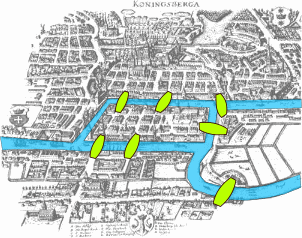
\includegraphics[width=\linewidth]{Pics/konigsberg1}
\end{columns}
\end{frame}

\begin{frame}{Skilgreiningar}
\begin{columns}
\column{0.5\textwidth}
\begin{itemize}
 \item Vegur í neti er röð af hnútum og leggjum sem tengjast saman
 \item Rás í neti er vegur þar sem upphafs- og endahnúturinn er sami hnúturinn
\end{itemize}
\column{0.5\textwidth}
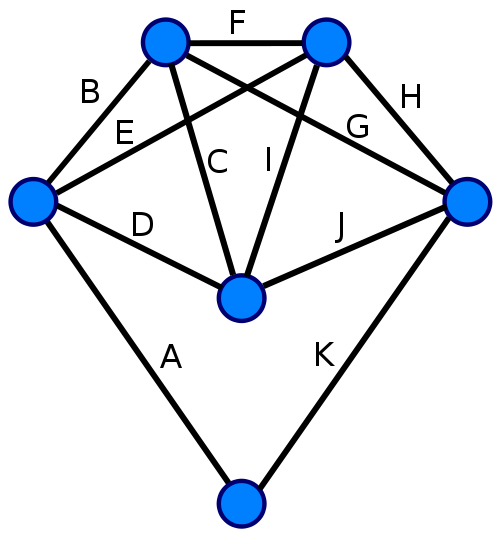
\includegraphics[width=\linewidth]{Pics/labelled-eulerian}
\end{columns}
\end{frame}

\begin{frame}{Brýrnar í Königsberg}
\begin{center}
Setjum vandamálið fram sem netavandamál
\end{center}

\begin{columns}
\column{0.48\textwidth}
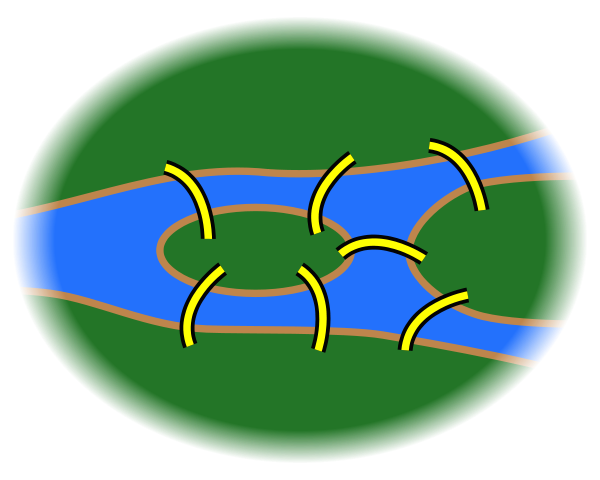
\includegraphics[width=\linewidth]{Pics/konigsberg2}
\column{0.04\textwidth}
$\to$
\column{0.48\textwidth}
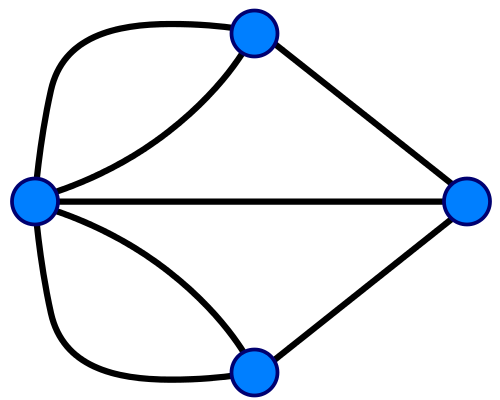
\includegraphics[width=\linewidth]{Pics/konigsberg3}
\end{columns}
\end{frame}

\begin{frame}{Fleiri skilgreiningar}
\begin{columns}
\column{0.5\textwidth}
\begin{itemize}
 \item Euler-vegur er vegur sem þekur alla leggi í neti nákvæmlega einu sinni
 \item Euler-rás er rás sem þekur alla leggi í neti nákvæmlega einu sinni
\end{itemize}
\column{0.5\textwidth}
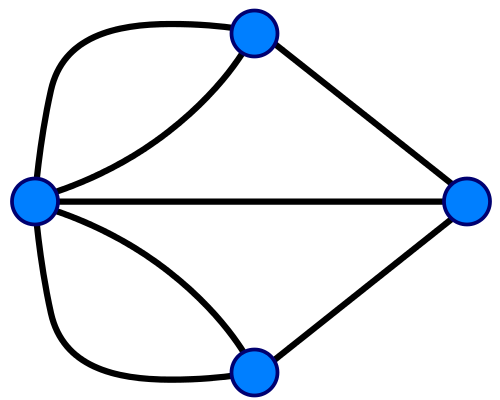
\includegraphics[width=\linewidth]{Pics/konigsberg3}
\end{columns}
\end{frame}

\begin{frame}{Staðhæfingar}
\begin{columns}
\column{0.5\textwidth}
\begin{itemize}
 \item Tengt óstefnt net hefur Euler-rás þá og því aðeins að allir hnútar í netinu hafi stig sem er slétt tala
 \item Tengt óstefnt net hefur Euler-veg þá og því aðeins að 0 eða 2 hnútar í netinu hafi stig sem er oddatala
\end{itemize}
\column{0.5\textwidth}
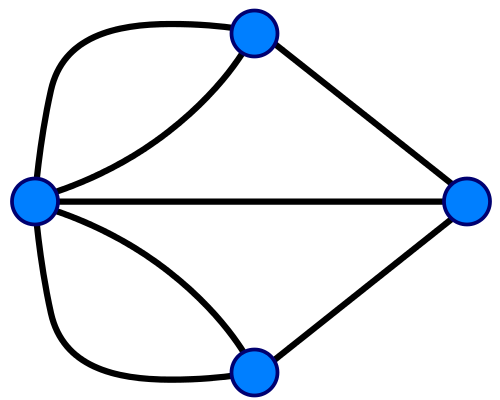
\includegraphics[width=\linewidth]{Pics/konigsberg3}
\end{columns}
\end{frame}

\section{Að finna vegi}

\begin{frame}{Að finna vegi}
\begin{itemize}
 \item Það að vinna sig í gegnum mjög skorðaða gagnagrind á borð við eintengdan lista eða tvíleitartré er ``einfalt''
 \item Til að finna leið í gegnum almennt net þurfum við að ákveða aðferð
 \item Skilgreinum upphafshnút og vinnum okkur út frá honum
\end{itemize}
\end{frame}

\begin{frame}{Breiðleit}
Hugmyndin í breiðleit: Skoðum nágranna. Notum biðröð til að ákvarða hvaða hnúta við skoðum næst.
\begin{center}
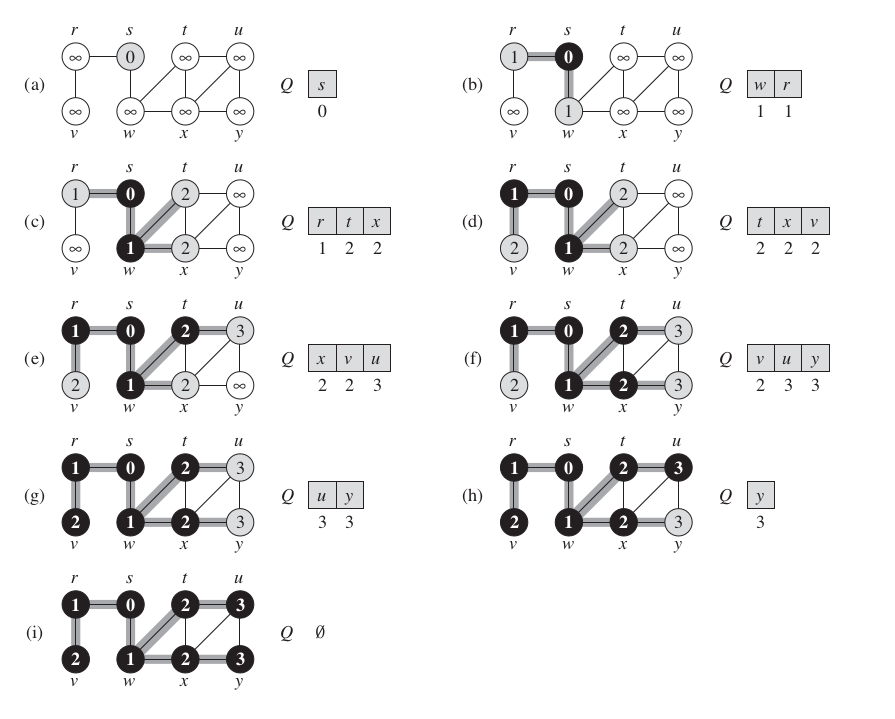
\includegraphics[width=0.8\textwidth]{Pics/bfs-example}
\end{center}
\end{frame}

\begin{frame}{Djúpleit}
Hugmyndin í breiðleit: Skoðum nágranna. Notum hlaða til að ákvarða hvaða hnúta við skoðum næst.
\begin{center}
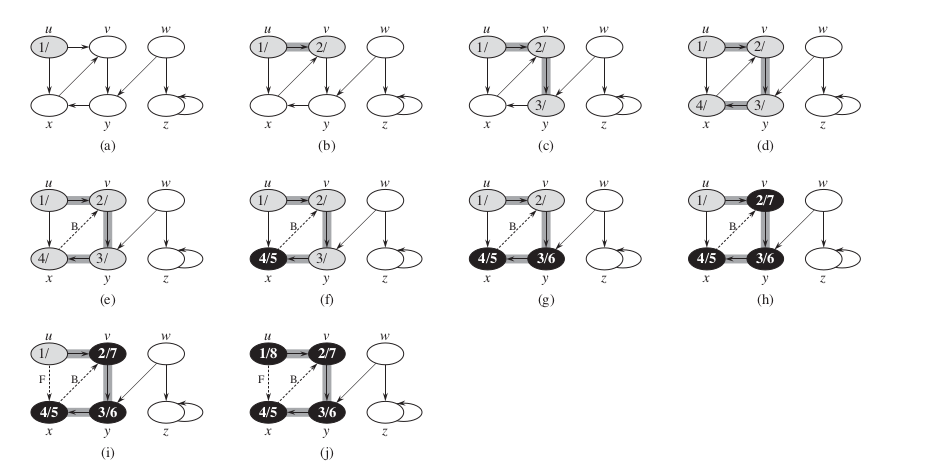
\includegraphics[width=\textwidth]{Pics/dfs-example}
\end{center}
\end{frame}

\begin{frame}
\href{http://qiao.github.io/PathFinding.js/visual/}{Ýmis leitarreiknirit á fleti}
\end{frame}


\end{document}
